\documentclass[22pt]{beamer}
\usepackage[orientation=portrait, size=custom, width=91.44, height=60.96,scale=1.2]{beamerposter} % 36in*2.5 = 90cm
\usepackage[absolute,overlay]{textpos}
\usepackage{bookmark} %pdflatex says to use this to avoid errors...
\usepackage{graphicx} %for including images
\graphicspath{{assets/images/}} %location of images
\usepackage{wrapfig} %wrap text around the images
\usepackage{listingsutf8}    %package for code environment; use this instead of verbatim to get automatic line break; use this instead of listings to get (•)
\usepackage{amsmath}
\usepackage{gensymb}
\usepackage[export]{adjustbox}
\usepackage[skins,theorems]{tcolorbox}
\usepackage{tikz}
\newcommand*\circled[1]{\tikz[baseline=(char.base)]{
            \node[shape=circle,draw,inner sep=2pt] (char) {#1};}}
\usepackage{array}
\usepackage{booktabs,adjustbox}
\usepackage{subcaption}
\usepackage{pgfplots}
%plot options
\pgfplotsset{width=7cm,compat=1.8}
\PassOptionsToPackage{gray}{xcolor}
% \usepackage{cite}
\usepackage[round]{natbib}
\defcitealias{ISTQB}{Hamburg and Mogyorodi, 2024}
\usepackage{fancyvrb}

\usetikzlibrary{shapes,shapes.geometric,arrows,fit,calc,positioning,automata,}
\usepackage{pgf-pie}

\usepackage{wrapfig}

%\mode<presentation>
%this doesn't seem to make any difference; leave for now for trying out
\usetheme{Berlin}
\definecolor{MacBlue}{rgb}{0.10196,0.22353,0.53725}
\definecolor{MacMaroon} {rgb}{0.47843, 0, 0.23137}
\definecolor{MacMaroon2} {rgb}{0.47451, 0, 0}
\definecolor{MacGray}{rgb}{0.50196,0.49804,0.51765}
\definecolor{MacMaroon3}{rgb}{00.47,0.2,0.31}
\definecolor{MacGold}{rgb}{1, 0.75,0.35}
\usecolortheme[named=MacMaroon2]{structure}
\setbeamertemplate{caption}[numbered]
\setbeamertemplate{navigation symbols}{}

% From https://tex.stackexchange.com/questions/201216/beamer-nested-lists-do-not-decrease-the-font-size
\setbeamerfont{itemize/enumerate subbody}{size=\normalsize} %to set sub-itemize size

\title{A New Taxonomy of Software Testing Approaches}
\subtitle{Seeking More Standardized Standards}
  \author[Crawford]{Samuel Joseph Crawford\newline \small crawfs1@mcmaster.ca} % \{schankuc, geiskkod, smiths, anandc\}
  \institute[McMaster University]{Department of Computing and Software, McMaster University} % $^\dagger$
  \date{April 22, 2023}

\begin{document}
%compile with pdflatex

%there is only one frame, because there is only one page; yeah, it's a poster
%textblock and block seem to work nicely to organize layout
\begin{frame}[fragile]

    \begin{textblock}{2}(0.7,1)
        
\includegraphics[height=8.5cm]{eng_logo.png}
    \end{textblock}

    \begin{textblock}{2}(13,0.55)
        
\includegraphics[height=12.5cm]{cas_logo.png}
    \end{textblock}

    \begin{textblock}{8}(4,1)
        \titlepage
    \end{textblock}

    \begin{textblock}{7.25}(0.5,3.6)

        %this needs help
        \begin{block}{\fontsize{37}{20}\selectfont Background}
            The first step to any formal process is understanding the underlying
            domain well. Therefore, a systematic and rigorous understanding of
            software testing approaches is needed to develop formal tools to test
            software. In my specific case, my motivation was seeing which kinds
            of testing could be generated automatically by Drasil, ``a framework
            for generating all of the software artifacts for (well understood)
            research software'' \citep{carette_drasil_2021}.

            \quad % needed for line break

            Most software testing ontologies seem to focus on the high-level
            testing process rather than the testing techniques themselves. For
            example, the terms and definitions \citep{TebesEtAl2020b} from
            TestTDO \citep{TebesEtAl2020a} mainly focus on parts of the testing
            process (e.g., test goal, test plan, testing role, testable entity)
            and how they relate to one another.
            \citet{UnterkalmsteinerEtAl2014} provide a foundation to allow one
            ``to classify and characterize alignment research and solutions
            that focus on the boundary between [requirements engineering and
                    software testing]'' but do not ``do[] not aim at providing a
            systematic and exhaustive state-of-the-art survey of [either domain]''
            (p.~A:2).
            \vspace{5mm}
        \end{block}

        \begin{block}{\fontsize{37}{20}\selectfont Methodology}
            \begin{itemize}
                \item If a taxonomy doesn't already exist, I should create one!
                      \begin{itemize}
                          \item I started with an ad hoc approach, focusing on
                                textbooks trusted at McMaster \\\citep{Patton2006,
                                    PetersAndPedrycz2000, vanVliet2000}
                          \item We then realized that this was too arbitrary, so
                                I then started from more established sources \\
                                (\citealp{IEEE2022, SWEBOK2024, SWEBOK2014,
                                    IEEE2017, ISO_IEC2023a}; \citetalias{ISTQB})
                          \item The goal of this approach is to iterate,
                                eventually revisiting the original textbooks,
                                until I build up enough knowledge to encounter
                                diminishing returns (ideally no returns!)
                      \end{itemize}
                \item Since there are many standardized documents about software
                      testing (or software in general), this should be trivial, no?
            \end{itemize}
            % \begin{figure}
            %     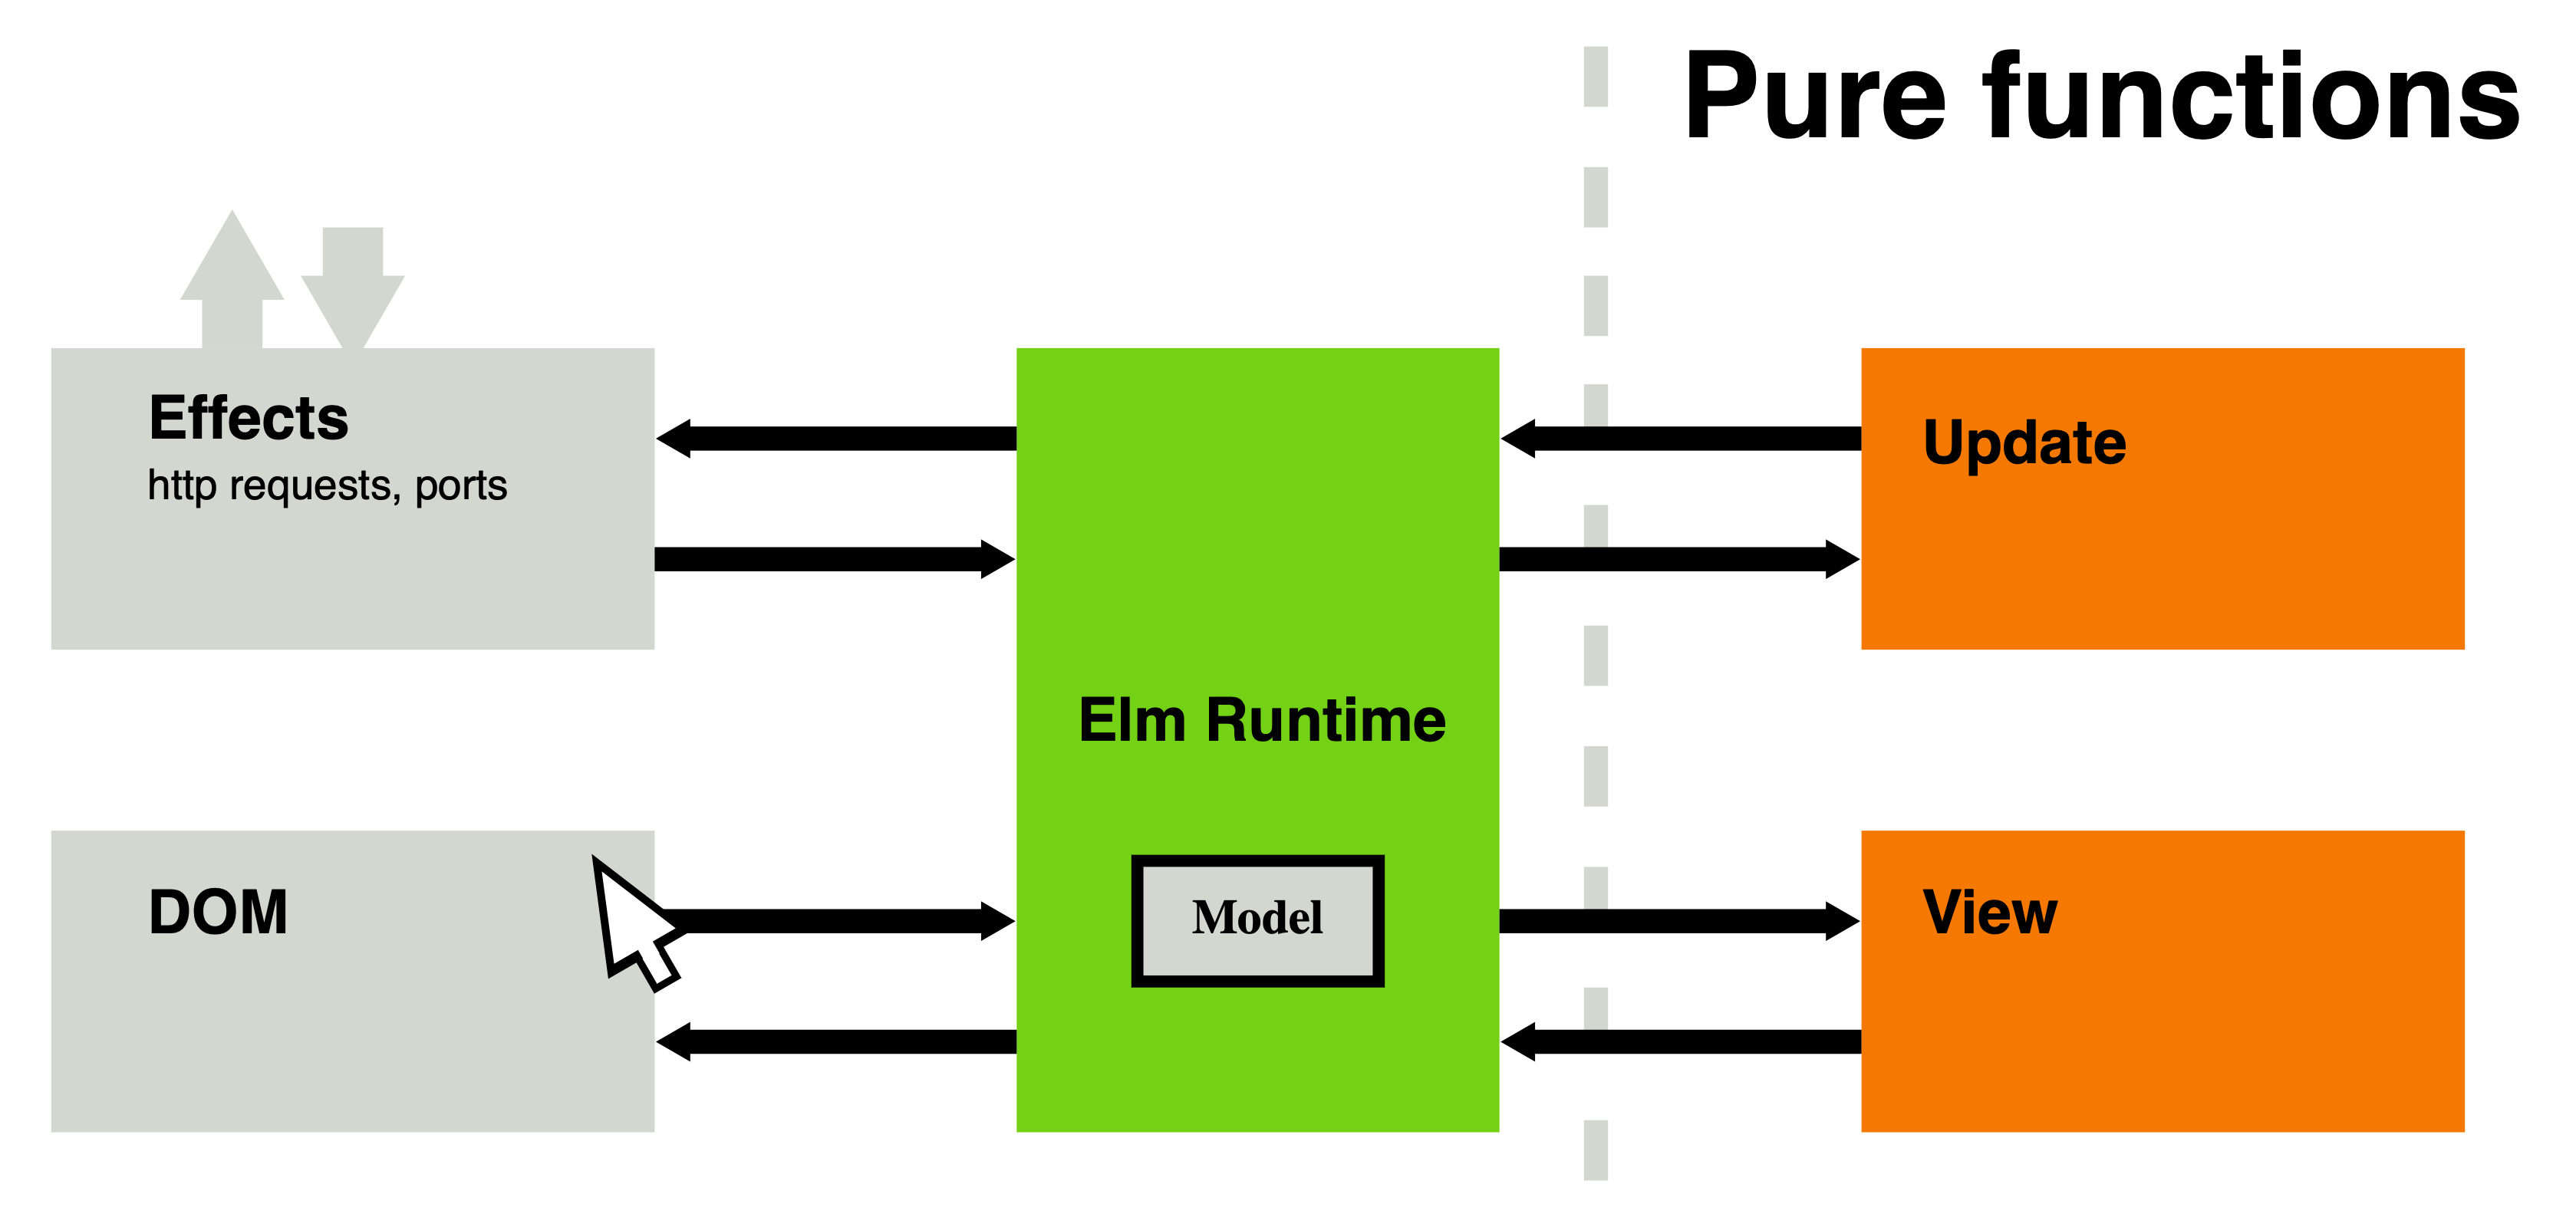
\includegraphics[height = 13cm]{TheElmArchitecture.png}
            %     \caption{The Elm Architecture consists of a \textit{model}, representing application data, a pure \textit{update} function to change the model in reaction to user events, called
            %         messages,
            %         and a pure \textit{view} function to render the application to the screen.}
            %     \label{Fig:TEA}
            % \end{figure}
            \vspace{5mm}
        \end{block}

        \begin{block}{\fontsize{37}{20}\selectfont My Findings}
            \vspace{5mm}
            {\fontsize{185}{20}\selectfont NO}
            \vspace{5mm}
        \end{block}
    \end{textblock}

    \begin{textblock}{7.25}(8.25,3.6)
        \begin{block}{\fontsize{37}{20}\selectfont Examples}
            \citep{IEEE2022} is a standard for general concepts related to
            software testing. However, it is not comprehensive. For example, as
            shown in Figure \ref{Fig:defs}, most (55 out of 99) testing
            approaches mentioned in this standard do not have an accompanying
            definition!

            \begin{figure}
                \begin{tikzpicture}[thick, scale=1.5, every node/.style={scale=0.8}]
                    \pie{44.4/Defined,
                        38.4/Undefined,
                        9.1/Present in another standard,
                        8.1/Present in previous version}
                \end{tikzpicture}
                \label{Fig:defs}
                \caption{Breakdown of testing approach definitions from \cite{IEEE2022}.}
            \end{figure}


            % \begin{figure}
            %     \begin{subfigure}{0.49\textwidth}
            %         \centering
            %         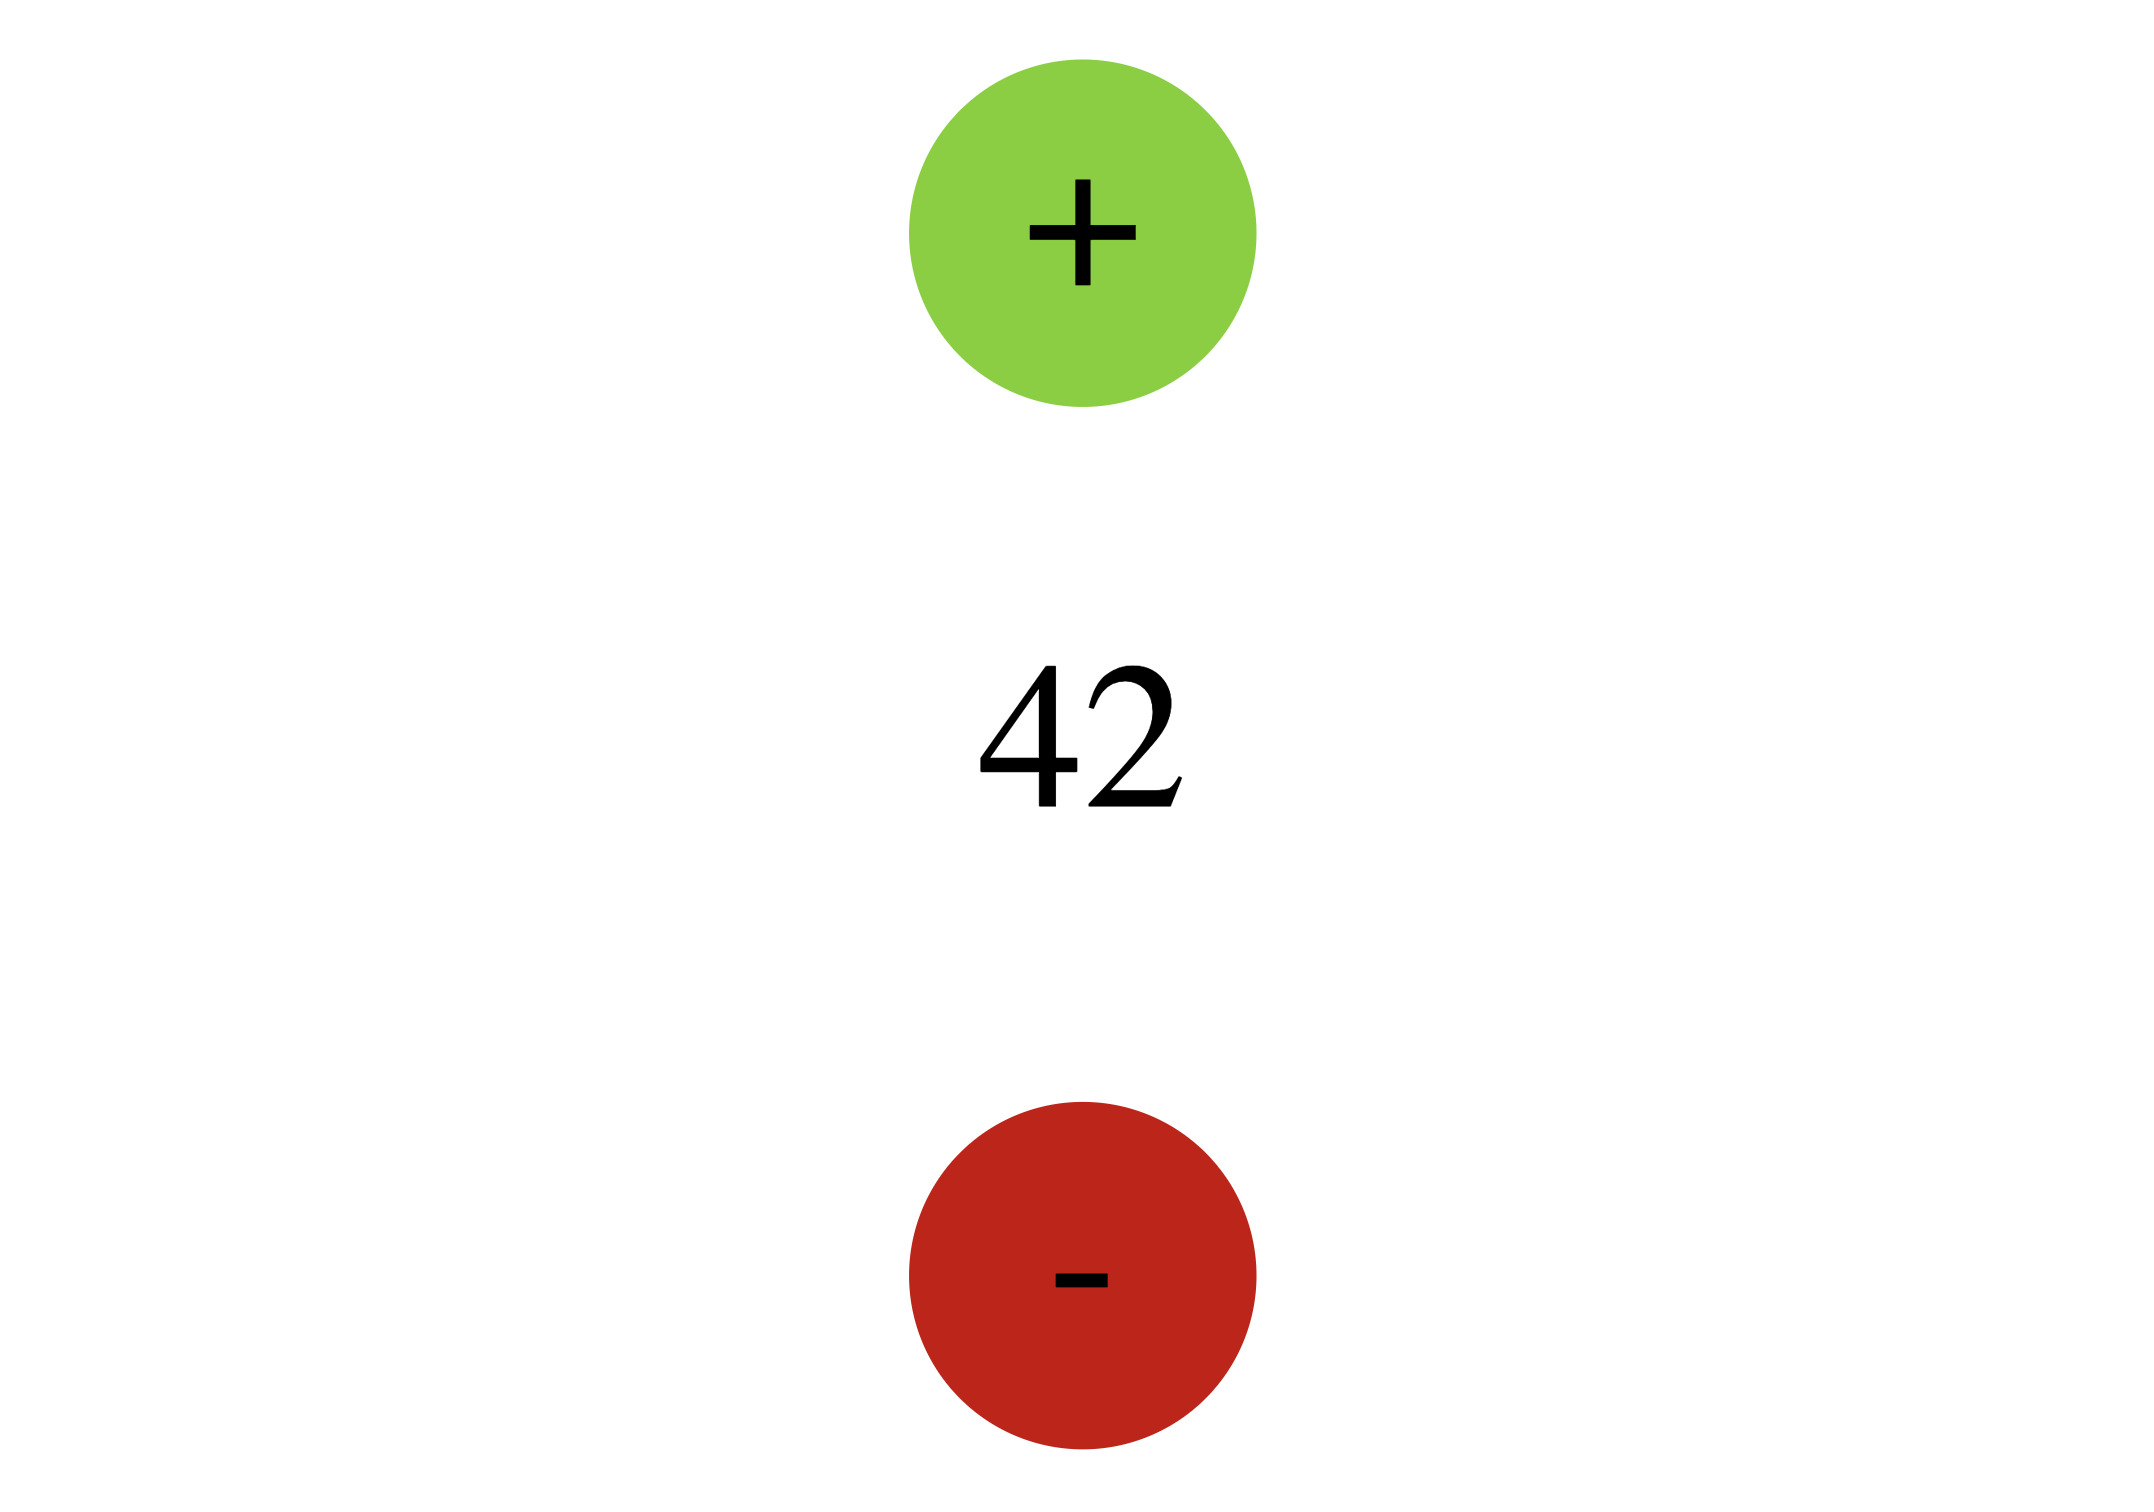
\includegraphics[height = 13.5cm,trim={0 5mm 0 5mm},clip]{IncDec.png}
            %         \caption{Example TEASync counting application}
            %         \label{Fig:Counter}
            %     \end{subfigure}
            %     \begin{subfigure}{0.49\textwidth}
            %         \centering
            %         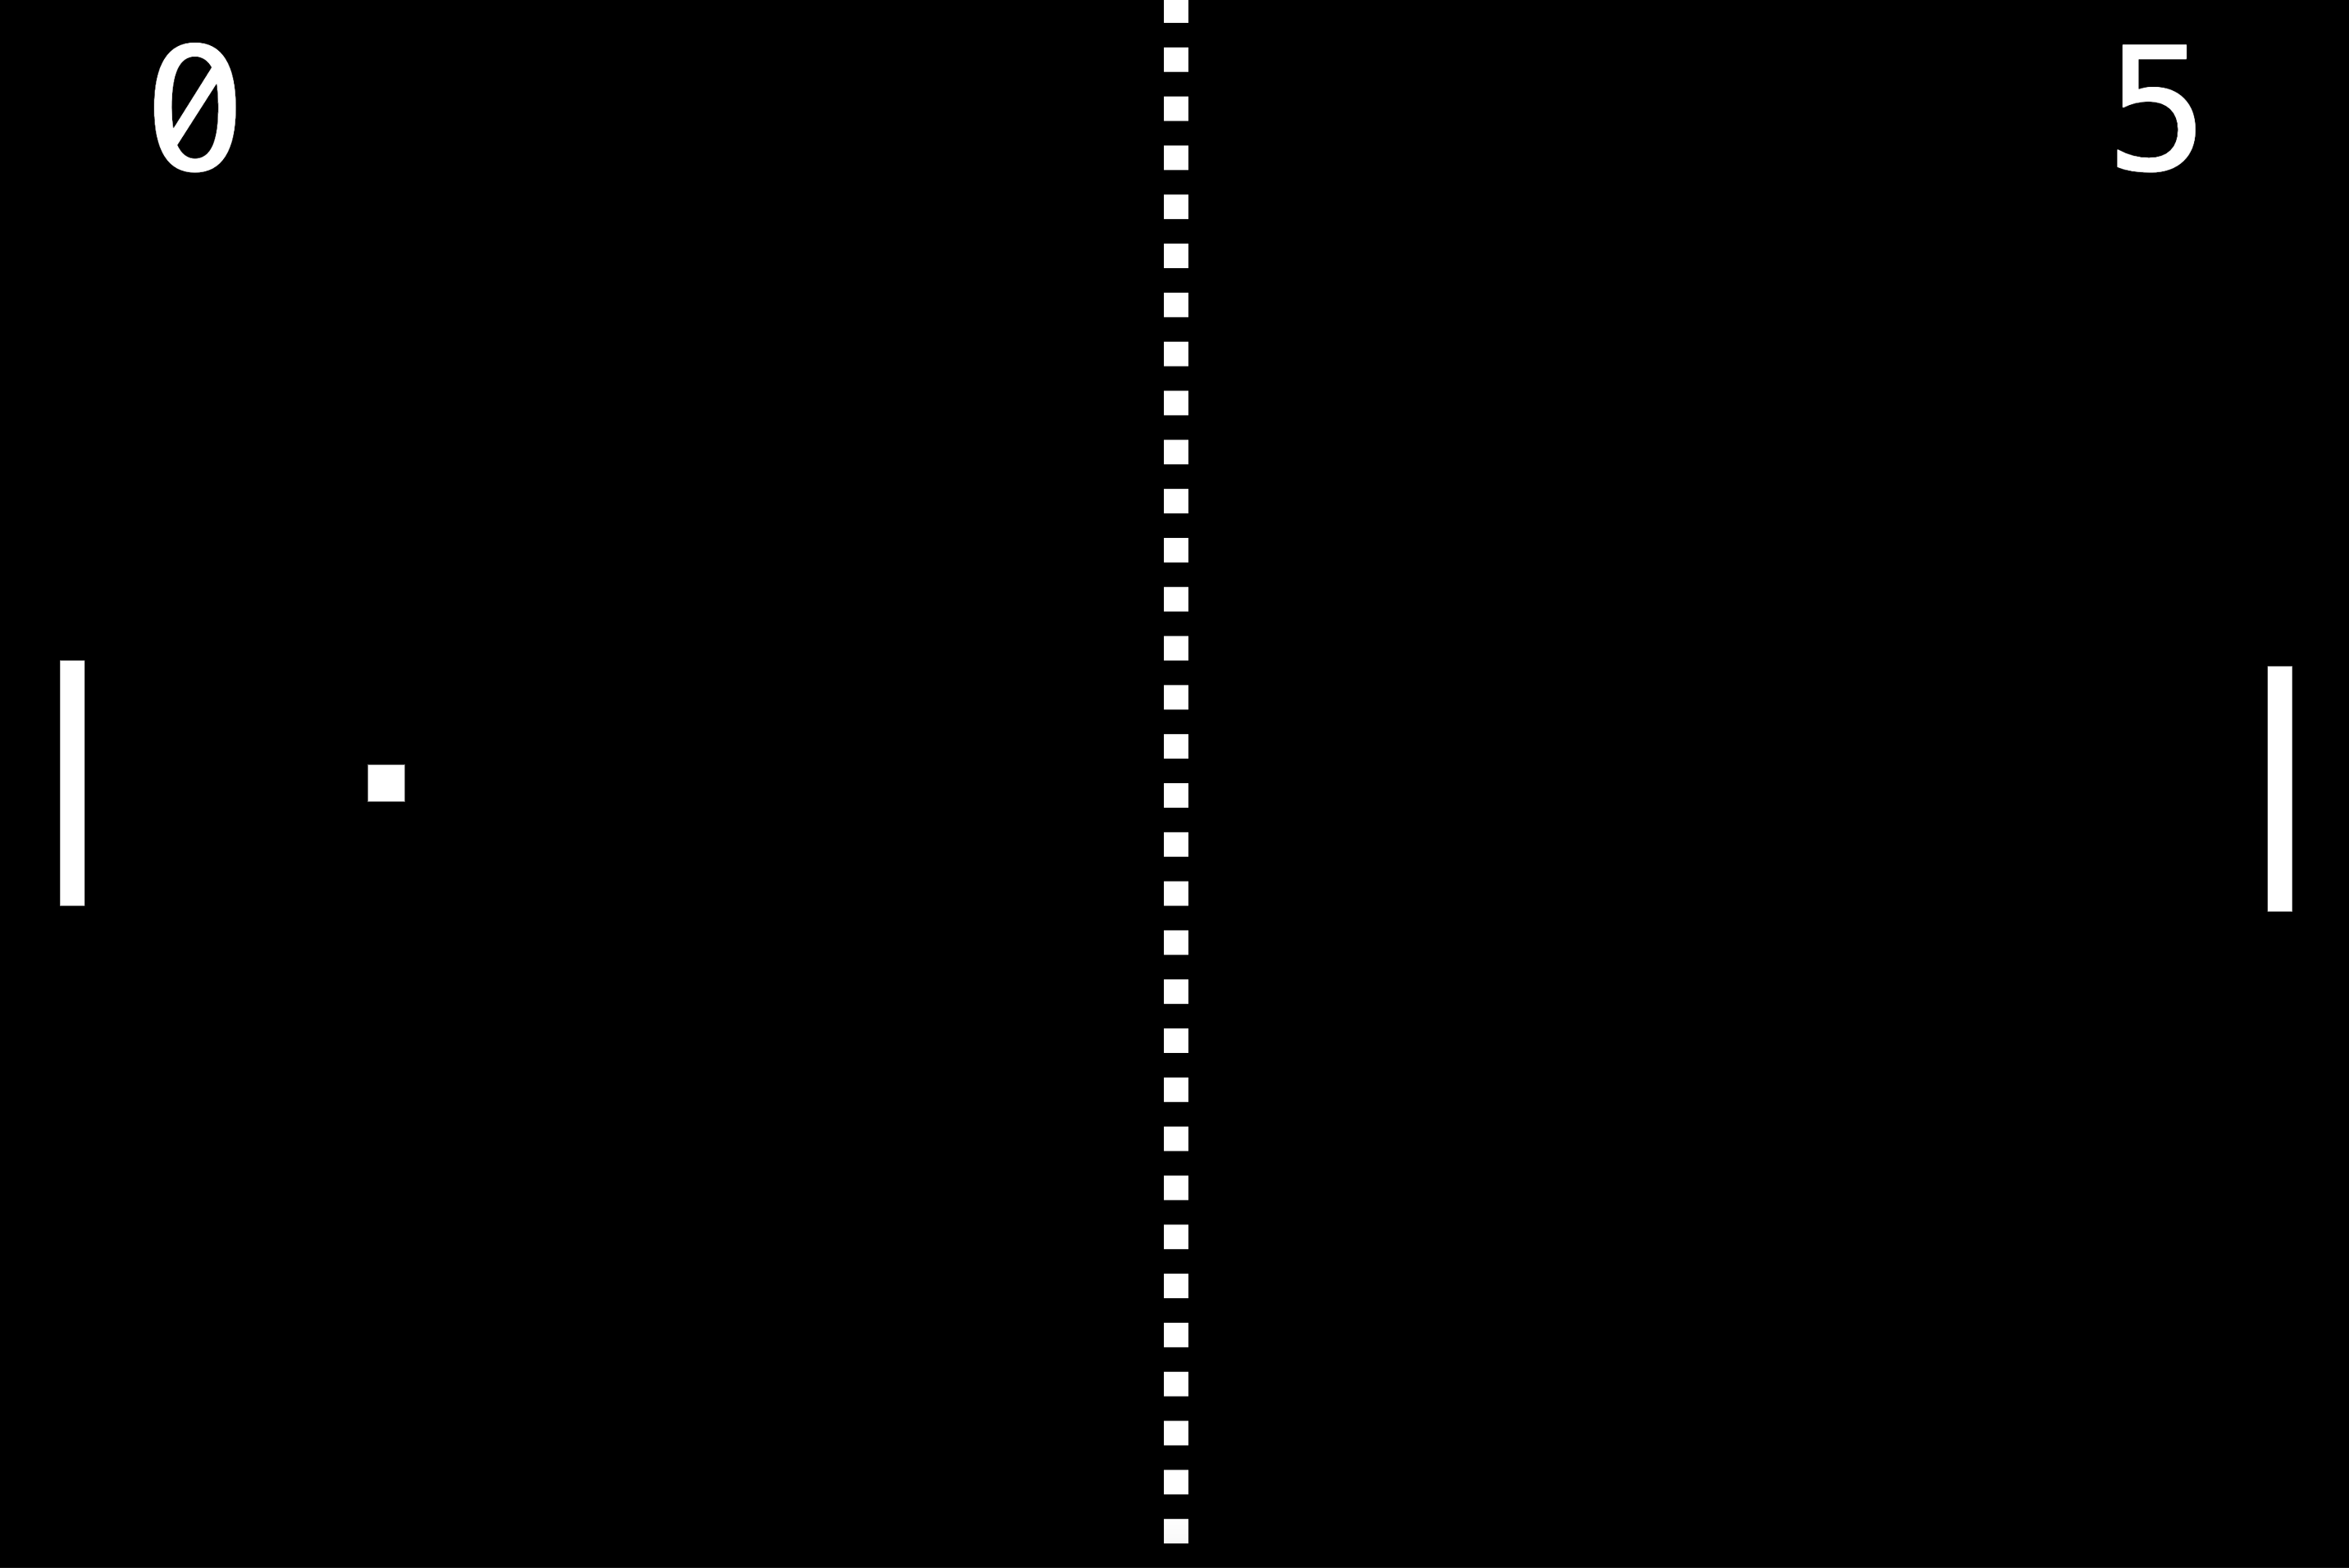
\includegraphics[height = 13.5cm]{Pong.png}
            %         \caption{Example TEASync multiplayer Pong game}
            %         \label{Fig:Pong}
            %     \end{subfigure}
            %     \caption{Example TEASync application user interfaces}
            % \end{figure}
            \vspace{-5mm}
        \end{block}

        \begin{block}{\fontsize{37}{20}\selectfont Conclusions \& Future Work}
            Leveraging the strictly-typed nature of Elm and its model-view-update architecture, we were able
            to create a simplified multi-user framework, requiring the programmer to write no server-side code. In addition to the upcoming pedagogical study, future work includes a data modelling extension allowing persistent, structured data, an
            authentication/authorization scheme, a binary data format to reduce network communication, and
            curriculum development for a TEASync-based summer camp.
        \end{block}

        % \begin{block}{\fontsize{37}{20}\selectfont References}
        % \scriptsize
        % \bibliographystyle{ieeetran}
        % \bibliography{bib}
        % \end{block}

        \begin{block}{\fontsize{37}{20}\selectfont References}
            \setbeamertemplate{bibliography item}{\insertbiblabel}
            \bibliographystyle{plainnat}
            % \bibliographystyle{ieeetr}
            {\fontsize{14}{15.75}\selectfont
                \bibliography{references}}
        \end{block}

        \begin{block}{\fontsize{37}{20}\selectfont Acknowledgments}
            We thank NSERC for CGS-M funding and the Government of Ontario for OGS funding.
        \end{block}

        % \begin{figure}[htbp]
        %     \centering
        %     
\includegraphics[height=5cm,trim={0 0 28.5cm 0},clip]{nserc-logo.jpg}
        %     \hspace{0.5cm}
        %     
\includegraphics[height=5cm,trim={16.5cm 0 0 0},clip]{ontario@2x-print.png}
        %     \hspace{0.5cm}
        %     
\includegraphics[height=5cm]{STaBLLogoWS.png}
        %     \hspace{0.5cm}
        %     
\includegraphics[height=5cm]{elm-logo.png}
        %     \hspace{0.5cm}
        %     
\includegraphics[height=5cm]{IHPLogo.png}

        % \end{figure}
    \end{textblock}

    % \begin{textblock}{5}(10.7,3.8)
    % \begin{figure}
    % 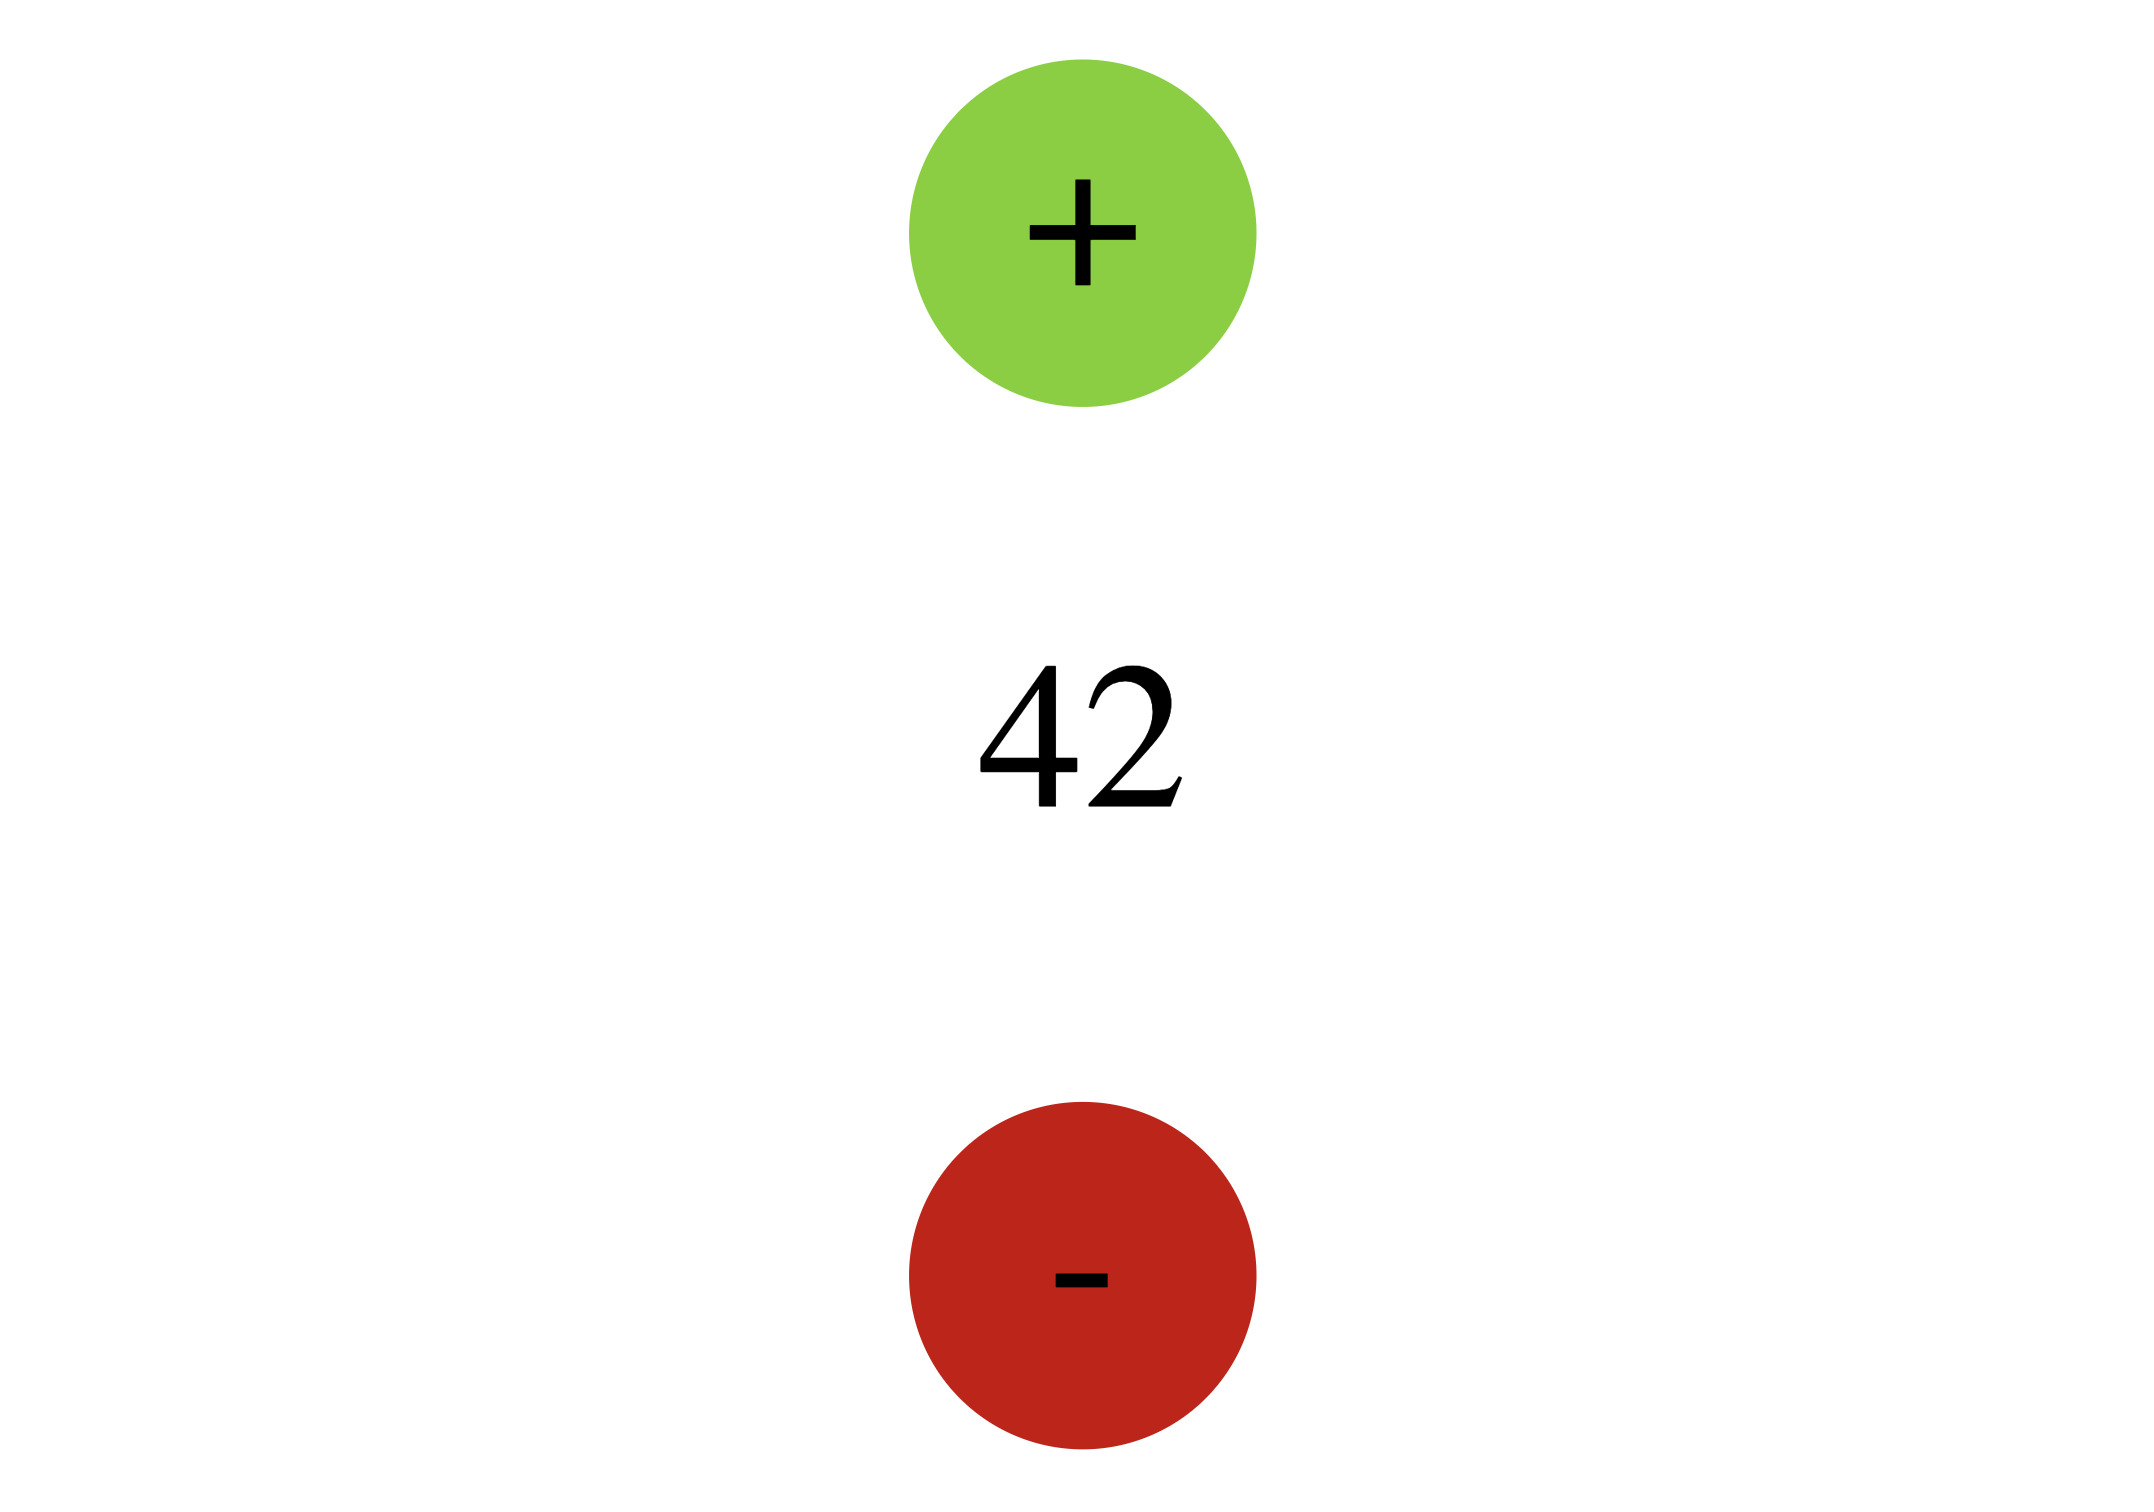
\includegraphics[height = 11cm]{IncDec.png}
    % \caption{Example TEASync counting application}
    % \label{fig:Counter}
    % \end{figure}
    % \end{textblock}

\end{frame}
\end{document}
